\documentclass{standalone}
\begin{document}

	\subsection{Lung Extraction}
	
	Lung extraction is the first step of the pipeline that is performed by homonymus script. As input the CT scan to process in each format supported by SimpleITK and will provide as output the isolated lung regions as default in '.nii' format.\\
	To achievement of the lung extraction involves 3 main steps: 
	  
	\begin{enumerate}
		\item \textbf{Pre-Processing} :  Which register the HU in a common space, crop the outliers, and de-noise the image;
		
		\item \textbf{Thresholding and reconstruction} : Which is the actual segmentation, that takes care to preserve all the intra-lung regions exept for the main bronchial structures.
		
		\item \textbf{Selection of lung} : allows the exclusion of all the extra-lung organs like intestine.
	\end{enumerate}

	
	\subsubsection{Pre-processing} 
	
	As I've said before, the $k$ constant in the HU definition (equation\,\ref{eq:HU}) may change according to the scan manufacturer or scan model. Moreover, during the scan acquisition, all the regions outside the CT tube aren't sampled, so to obtain a square $N\times N$ image for each slice some padding values are added, which different values according to the scan manufacturer: for instance in the CT scan in \figurename\,\ref{fig:Pre-Processing}(a) the padding value is $-3000 HU$ and the air value is $-1024$. The first thing to do is to make the padding value and the air value equal for each scan considered and shift them to $0$, because for the de-noising operation we need to works with unsigned int 16-bit gray scale image.\\
	May also happen that some Hu are out of range, that because some patients may have metallic prosthesis that make the so called \textit{metallic artifacts}. However we haven't to worry about this kind of artifacts because they will involves only body regions and not the lung ones,and so are removed during this step.
	In \figurename\,\ref{fig:Pre-Processing}(b) we can observe the histogram of the same scan after this pre-processing step, it is clear that both the padding and air values are set equal and shifted to zero, making positives all the other units.
	
	\begin{figure}[h]
		\centering
		\subfigure[Histogram of a CT scan before registration]
			{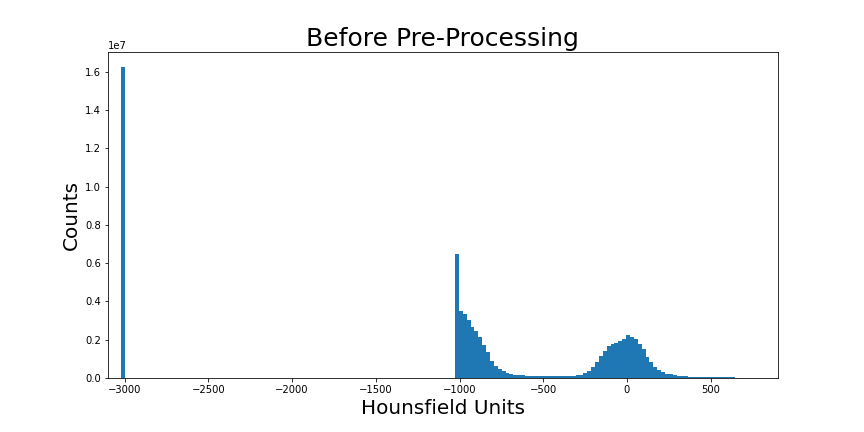
\includegraphics[scale=.4]{HU_before_rescaling.png}}
		%\hspace{1mm}
		\subfigure[Histogram of a CT scan after the registration]
			{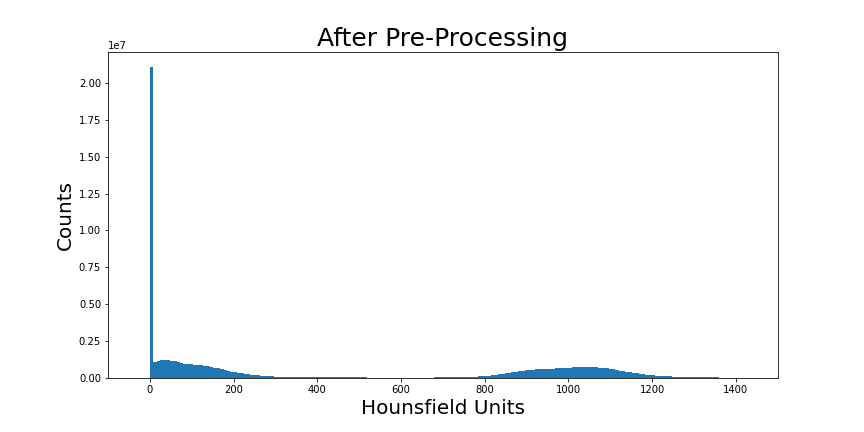
\includegraphics[scale=.4]{HU_after_rescaling.png}}
		\label{fig:Pre-Processing}\caption{Histogram of voxel values before and after the pre-processing. We can observe that before the pre processing there are some HU out of range, which are the values used to fill the regions outside the tube, and the air value is around $-1000\,HU$ according to HU definition. After the rescaling we can observe that all the values are non-negatives.}
	\end{figure}
	
	
	
	Before starting the actual lung segmentation, we need to performs a de-noising operations, which allow us to increase the differences between the GL of the body regions, and to sharp the edges. According to the procedure described in ~\cite{ART:Abdullah}, I've used the bit plane slices. This approach allows to use the way in which each numerical values is stored in the computer by converting  each values with its binary representation, this allows us to construct an image in which each voxel intensity is given only by the bits representing the regions multiplied by their significance.
	
	\begin{figure}[h]
		\centering
			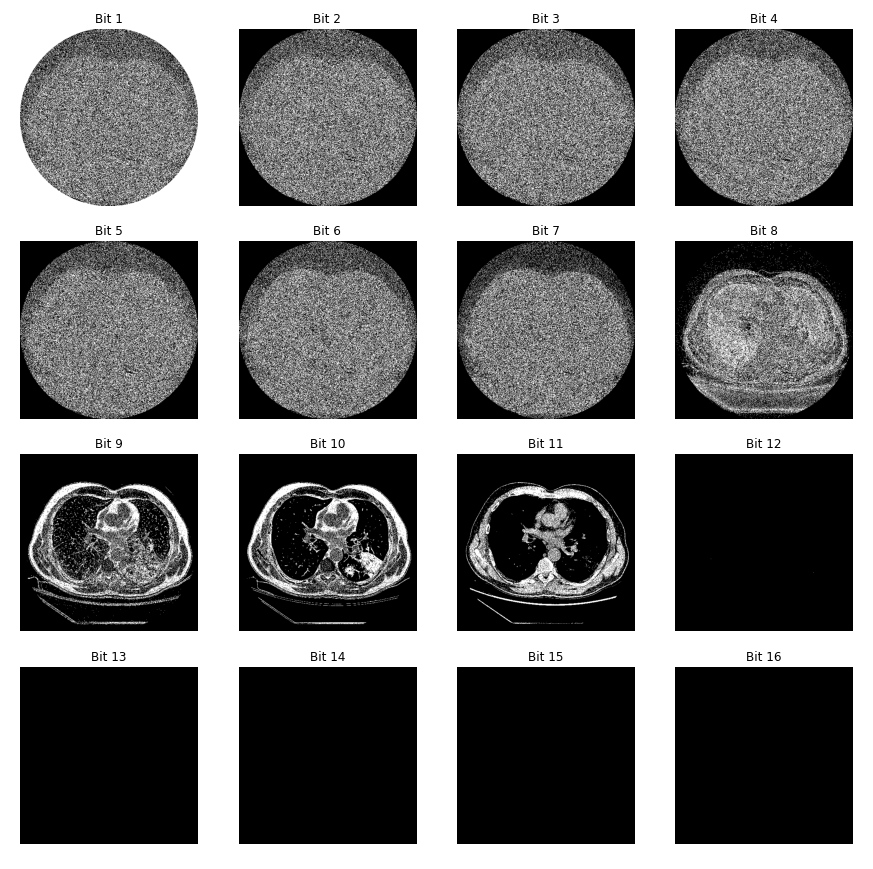
\includegraphics[scale=.45]{bit_plane_slices.png}
		\label{fig:BinaryRepr}\caption{Images corresponding to each one of the 16 bits. The image form the $1\,st$ to the $8\,th $ bit carry only noise, and the images form the $12\,th$ to the $161,th$ doesn't  contains any information. The de noised image is composed of the $9\,th,\,10th,\,and 11\,th$ bits times their significance. }
	\end{figure}

	In \figurename\,\ref{fig:BinaryRepr} are displayed the images for each bit. As we can see all the bits from the 1st to the 11th doesn't carry any useful information but only noise, on the other and the bits from the 12th to the 16th aren't used in the image representation. In the end the de-noised image is constructed by using only the 9th, 10th and 11th bits times their significance that is defined as $significance = 2^{bit}$
	In this way we have constructed an image in which the noise is highly reduced and the different regions are well separated.\\
	After these procedures the scan is ready for the actual lung segmentation.
	
	

	\subsubsection*{Thresholding and reconstruction}
	
	For the actual lung segmentation we have found that the most suitable technique is simply a global fixed threshold, since now the GL of the different body regions are well separated. This allow us to include all the intra-lung regions including the GGO, which are usually dropped if an adaptive threshold, like otsu, is performed.
	However after this process  also extra lung regions, like intestine are segmented as lung. This is the reason why we need the last step to select only the lung.
	
	\subsubsection*{Lung Selection}
	
	In \figurename\,\ref{fig:lungSelection}(a), I've reported a 3D reconstruction of the selected regions after the second step. As we can see the intestine is selected with the lung, which are connected by trachea and bronchi. 
	
	
	
	\begin{figure}[h]
		\centering
		\subfigure[]
		{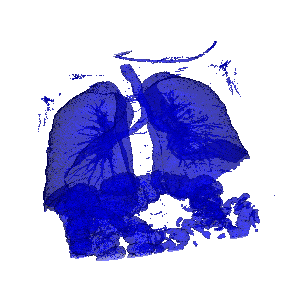
\includegraphics[scale=.65]{before_cc.png}}
		%\hspace{1mm}
		\subfigure[]
		{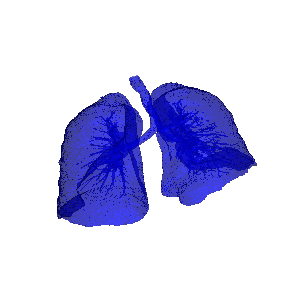
\includegraphics[scale=.65]{after_cc.png}}
		\label{fig:lungSelection}\caption{3D rendering of the selected lung structure. In figure (a) we can see the volume selected after the threshold. It possible to see that also the intestine is selected along with extra lung regions. In figure (b) the selected volume after the connected compoents. We can obseve how all the extra lung regions are correctly removed.} 
	\end{figure}
	
	On the other end the intestine is disconnected from the lung regions, since are structures anatomically disconnected. So we can use this characteristics to select only the lung. To perform this step I've used a suitable function from SimpleITK, which allow us to found the connected components by considering the whole image tensor, this means that we are able to found the connected components by considering all the 3 dimensions. At the end of the process, the components with the higher volume is the one corresponding to the lung and trachea regions, so we can simply select this component to achieve a correct selection of lung, as we see in \figurename\,\ref{fig:lungSelection}(b).
	
	\subsubsection*{Motion Artifact Removal}
	
	Once we have found a mask for the lung, we have to manage the motion artifacts. This artifacts are related to cardiac or respiratory motion, and interfere with the identification of infection areas, since they are identified like ground glass regions.  In this step we remove this kind of artifacts in order to reduce the number o false positives.\\ As we can see in  \figurename\,\ref{fig:Motion} this kind of artifacts are usually located near lung or heart regions and have an elongated form. The application of an hybrid hessian filter allow us to compute the contiguos edges, and in this way we are able to create a mask for the lung regions. However this method is not precise and can remove also interesting lung regions, so after that a reconstruction process is performed.\\
	
	\begin{figure}[h!]
		\centering
			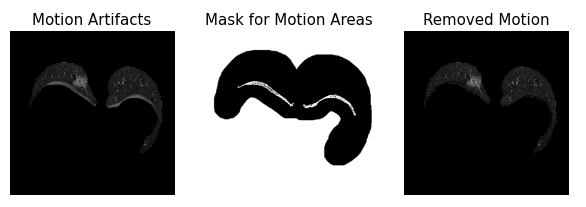
\includegraphics[scale=1.5]{Motion.png}
			\caption{From left to right the image with motion artifacts, the created mask and the image after the removal}
			\label{fig:Motion}
	\end{figure}
	
	
	In this way a lung mask is created and its applied to the pre-process image. The results will be saved in '.nii' format, which allows to preserve the spatial information about the voxel.
	
	
	
		
\end{document}